\documentclass{beamer}
\usepackage[utf8]{inputenc}
\usepackage{hyperref}

\usepackage{utopia}

\usetheme{Madrid}
\usecolortheme{default}

%------------------------------------------------------------
\title[JURECA]
{JURECA}

\subtitle{First modular supercomputer worldwide}

\author[Claudio Scheer]
{Claudio~Scheer\inst{1}}

\institute[PUCRS]
{
  \inst{1}%
  Master's Degree in Computer Science\\
  Pontifical Catholic University of Rio Grande do Sul - PUCRS
}

\date[June 2020]
{Parallel Architectures, June 2020}
%------------------------------------------------------------


%------------------------------------------------------------
\AtBeginSection[]
{
  \begin{frame}
    \frametitle{Table of Contents}
    \tableofcontents[currentsection]
  \end{frame}
}
%------------------------------------------------------------


\begin{document}

\frame{\titlepage}

%---------------------------------------------------------
\begin{frame}
  \frametitle{Table of Contents}
  \tableofcontents
\end{frame}
%---------------------------------------------------------


%---------------------------------------------------------
\section{Curiosities}

\begin{frame}
  \frametitle{Organization}

  \begin{itemize}
    \item Forschungszentrum Jülich is a interdisciplinary research centre in Germany;
    \item Institute for Advanced Simulation (IAS);
    \item Jülich Supercomputing Centre (JSC);
          \begin{itemize}
            \item Supercomputing centre since 1987;
          \end{itemize}
  \end{itemize}
\end{frame}

\begin{frame}
  \frametitle{Managed supercomputers}
  \begin{itemize}
    \item JUSUF;
    \item JUWELS (position 31\footnote{November 2019 ranking.});
          \begin{itemize}
            \item Helped Google demonstrate the quantum supremacy~\href{https://www.fz-juelich.de/SharedDocs/Pressemitteilungen/UK/EN/2019/2019-10-23-quantum-Supremacy.html}{(source)};
                  \begin{itemize}
                    \item Quantum computer: 200 seconds;
                    \item Fastest supercomputer: 10.000 years;
                  \end{itemize}
          \end{itemize}
    \item JURECA (position 56\footnotemark[\value{footnote}]);
          \begin{itemize}
            \item The name is short for Jülich Research on Exascale Cluster Architectures;
          \end{itemize}
  \end{itemize}
\end{frame}

\begin{frame}
  \frametitle{JURECA}
  \begin{itemize}
    \item 2015-04: begins to operate the cluster;
    \item 2017-11: included a buster module;
    \item First modular supercomputer worldwide~\href{https://www.fz-juelich.de/SharedDocs/Pressemitteilungen/UK/EN/2017/2017-11-13-jureca-booster.html}{(source)};
  \end{itemize}
\end{frame}
%---------------------------------------------------------


%---------------------------------------------------------
\section{Architecture}

\begin{frame}
  \frametitle{JURECA Cluster}
  \begin{columns}[T]
    \begin{column}{.5\textwidth}
      \begin{itemize}
        \item Dual-socket Intel Xeon E5-2680 v3 Haswell
        \item NVIDIA K40 and K80 GPUs
        \item 128/256/512 GiB memory per node (DDR4 @ 2133 MHz)
        \item 1884 compute nodes $\to$ 45.216 cores
        \item InfiniBand EDR (100 Gbps per link and direction)
      \end{itemize}
    \end{column}
    \begin{column}{.5\textwidth}
      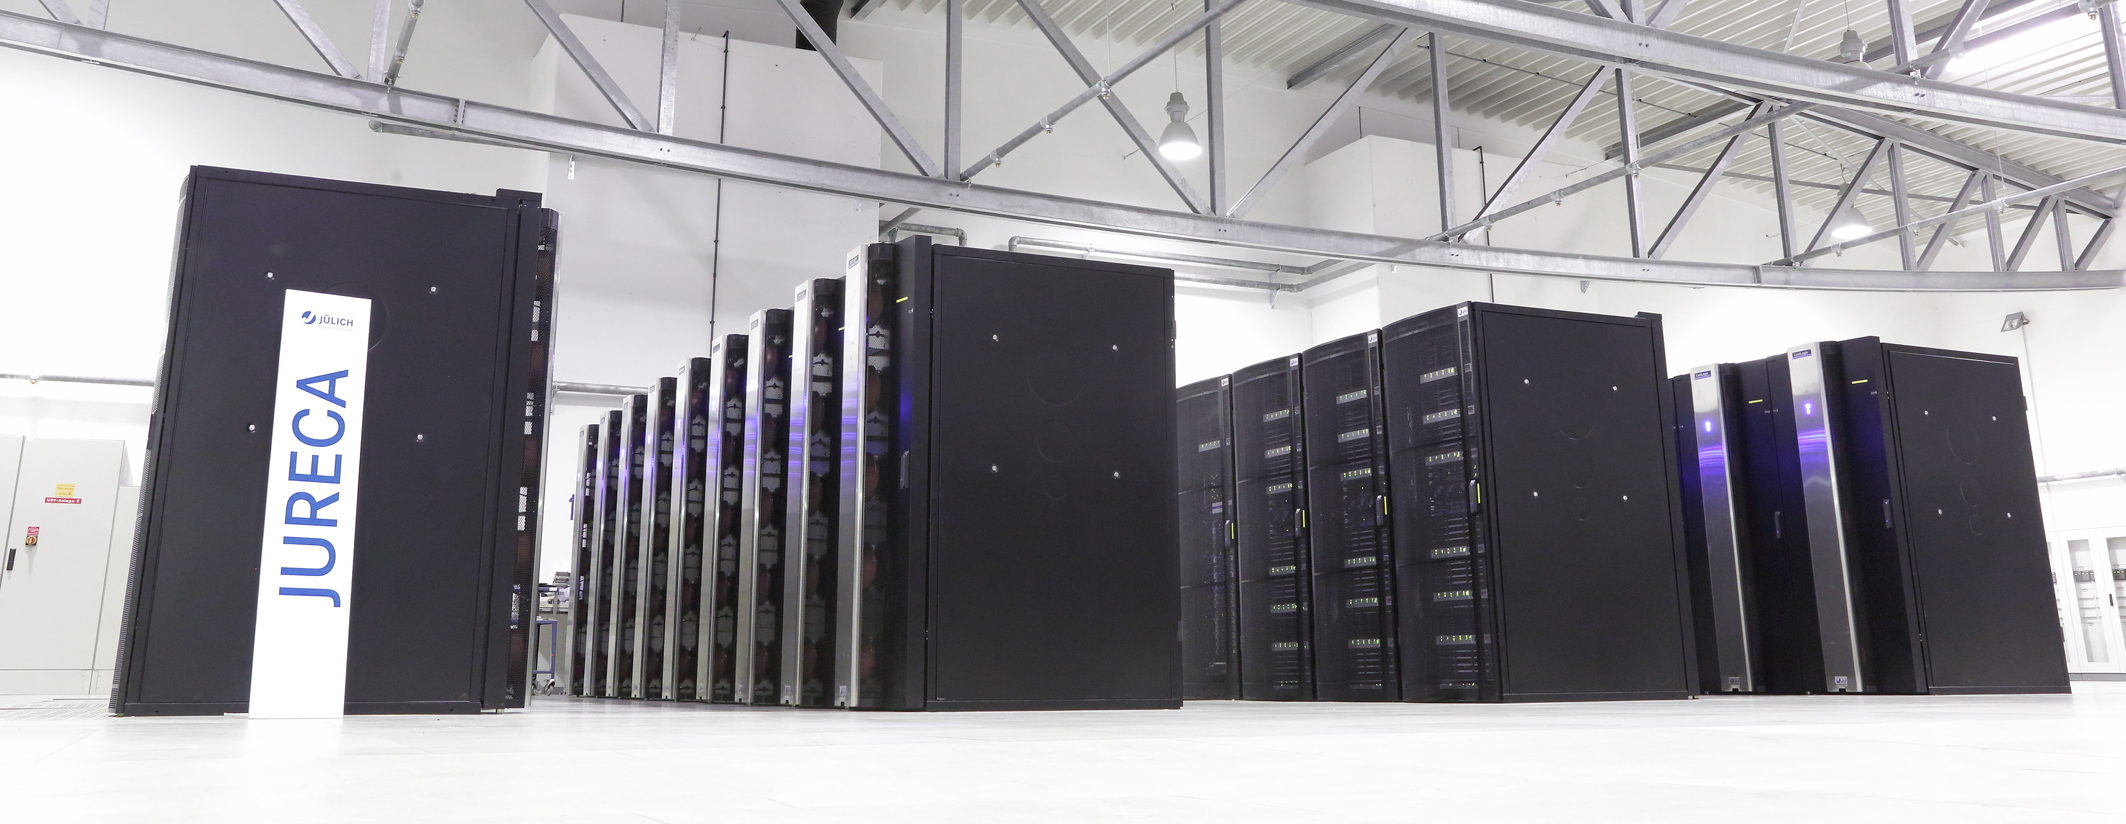
\includegraphics[width=\textwidth]{./images/jureca-cluster.jpeg}
    \end{column}
  \end{columns}
\end{frame}

\begin{frame}
  \frametitle{JURECA Buster}
  \begin{columns}[T]
    \begin{column}{.5\textwidth}
      \begin{itemize}
        \item asdaf
      \end{itemize}
    \end{column}
    \begin{column}{.5\textwidth}
      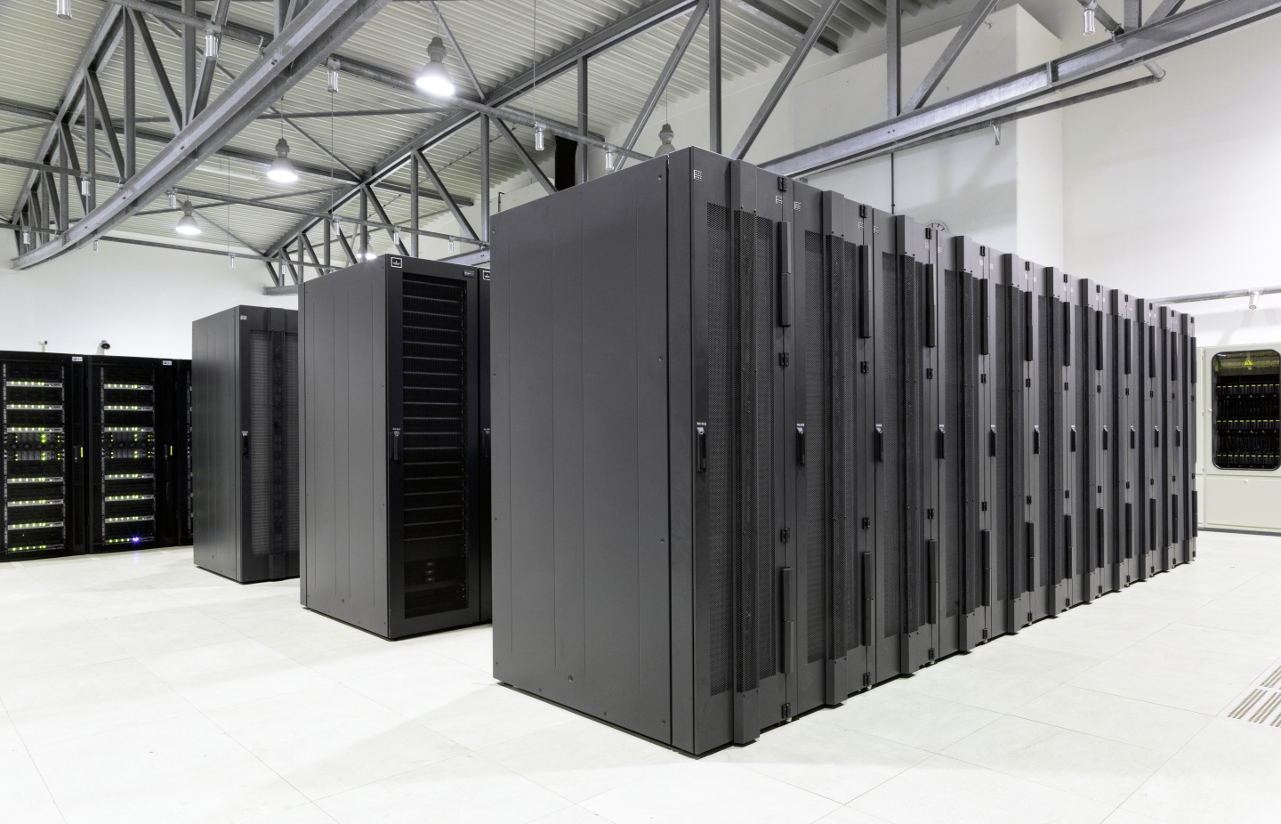
\includegraphics[width=\textwidth]{./images/jureca-buster.jpeg}
    \end{column}
  \end{columns}
\end{frame}

\begin{frame}
  \frametitle{Sample frame title}

  In this slide, some important text will be
  \alert{highlighted} because it's important.
  Please, don't abuse it.

  \begin{block}{Remark}
    Sample text
  \end{block}

  \begin{alertblock}{Important theorem}
    Sample text in red box
  \end{alertblock}

  \begin{examples}
    Sample text in green box. The title of the block is ``Examples".
  \end{examples}
\end{frame}
%---------------------------------------------------------


%---------------------------------------------------------
%Two columns
\begin{frame}
  \frametitle{Two-column slide}

  \begin{columns}

    \column{0.5\textwidth}
    This is a text in first column.
    $$E=mc^2$$
    \begin{itemize}
      \item First item
      \item Second item
    \end{itemize}

    \column{0.5\textwidth}
    This text will be in the second column
    and on a second tought this is a nice looking
    layout in some cases.
  \end{columns}
\end{frame}
%---------------------------------------------------------

\section{Classifications}

%---------------------------------------------------------
%Changing visivility of the text
\begin{frame}
  \frametitle{Sample frame title}
  This is a text in second frame. For the sake of showing an example.

  \begin{itemize}
    \item<1-> Text visible on slide 1
    \item<2-> Text visible on slide 2
    \item<3> Text visible on slides 3
    \item<4-> Text visible on slide 4
  \end{itemize}
\end{frame}

%---------------------------------------------------------


\section{Other resources}

%---------------------------------------------------------
\begin{frame}
  \frametitle{Other resources}

  \begin{itemize}
    \item \href{https://www.youtube.com/watch?v=7h6mYU2HDTA}{Time lapse video of the installation}
    \item \href{https://www.fz-juelich.de/ias/jsc/EN/Home/home_node.html}{Jülich Supercomputing Centre}
  \end{itemize}
\end{frame}

%---------------------------------------------------------

\end{document}